\chapter*{Pembuatan Aplikasi Menggunakan Apex}
\section{Memasukkan Tabel}
\par
Berikut merupakan cara-cara membuat aplikasi menggunakan APEX.
\begin{enumerate}
\item \textbf{Buka Website Apex terlebih dahulu}
\begin{figure}[H]
    \centering
    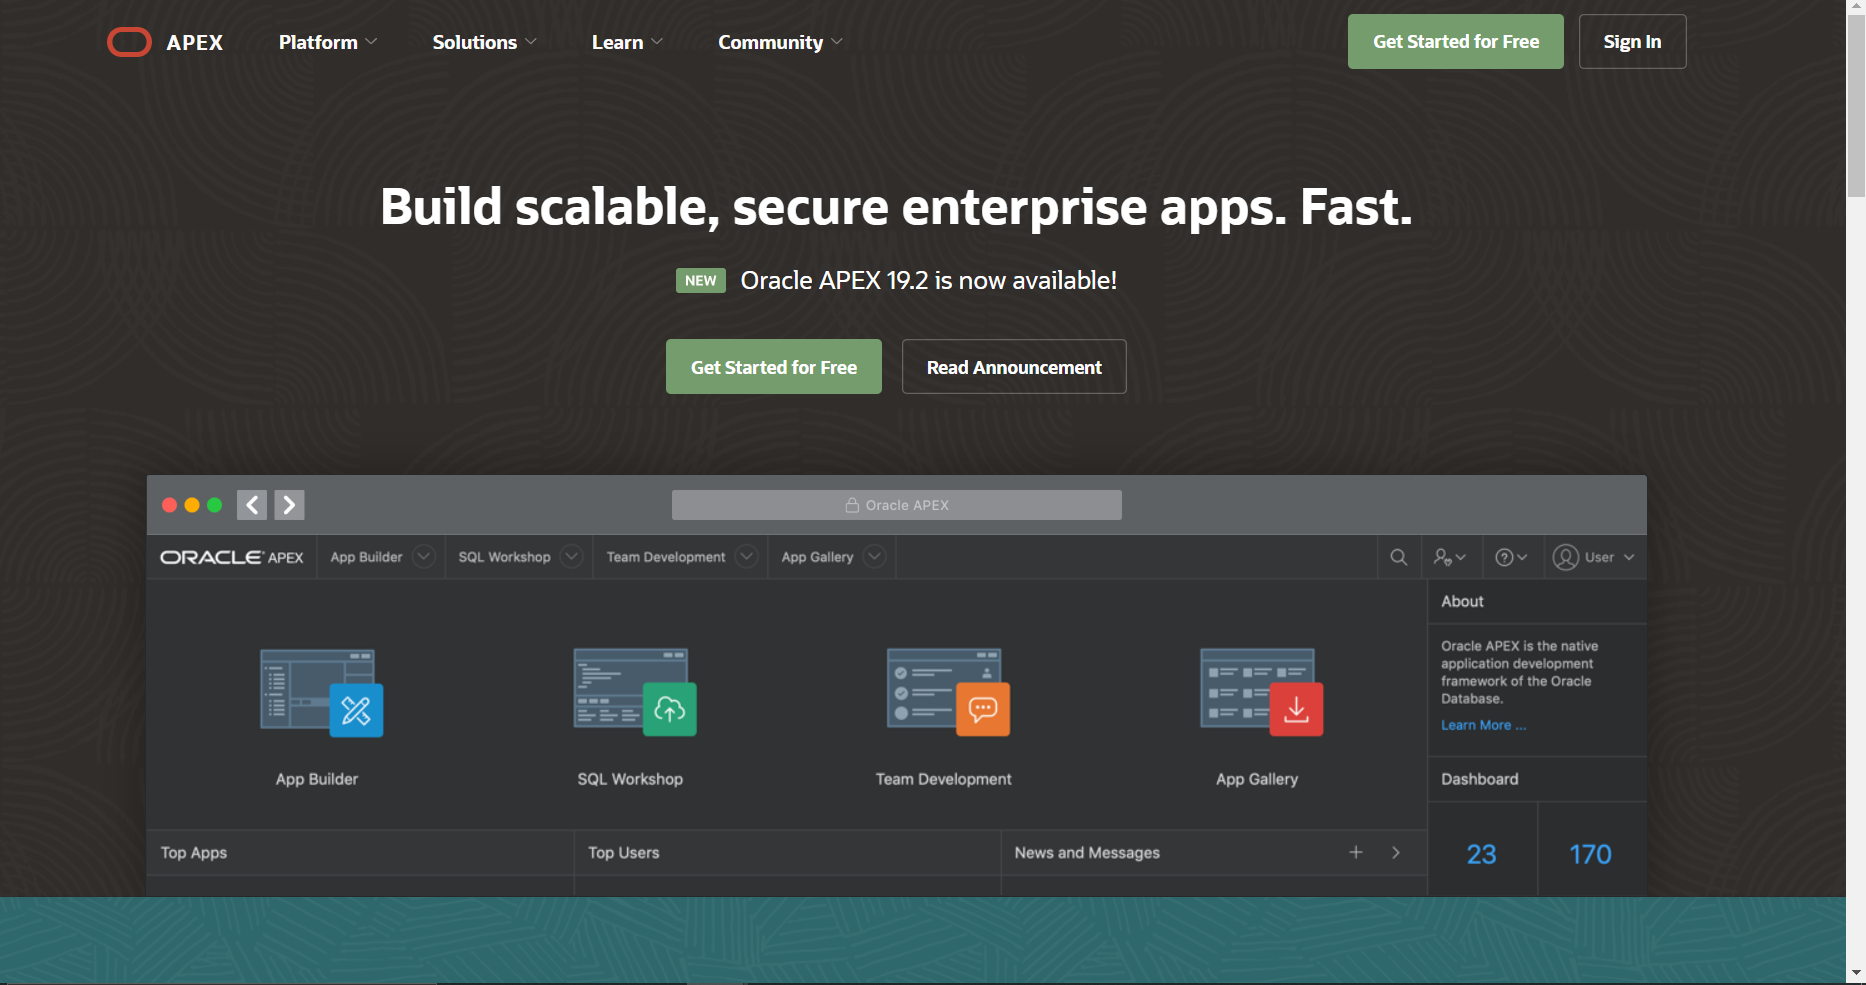
\includegraphics[scale=0.3]{figures/1.png}
    \label{1}
\end{figure}

\item \textbf{Setelah itu akan muncul form untuk sign in, Dikarenakan kita belum memiliki workspace, maka pilih opsi \textbf{Request a Workspace}}
\begin{figure}[H]
    \centering
    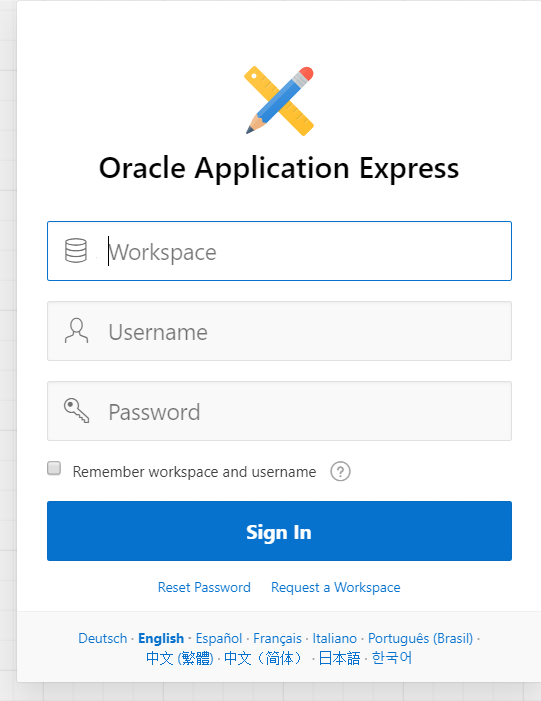
\includegraphics[scale=0.3]{figures/2.png}
    \label{2}
\end{figure}

\item \textbf{Masukkan data diri anda}
\begin{figure}[H]
    \centering
    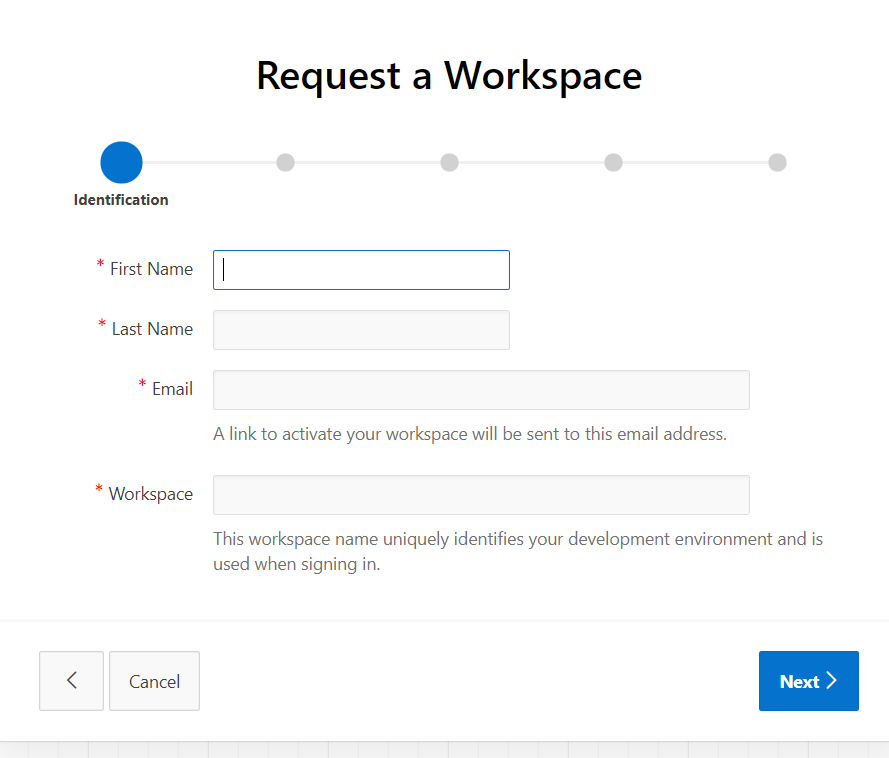
\includegraphics[scale=0.3]{figures/3.png}
    \label{3}
\end{figure}


\item \textbf{Isi beberapa survey yang disediakan oleh oracle}\begin{figure}[H]
    \centering
    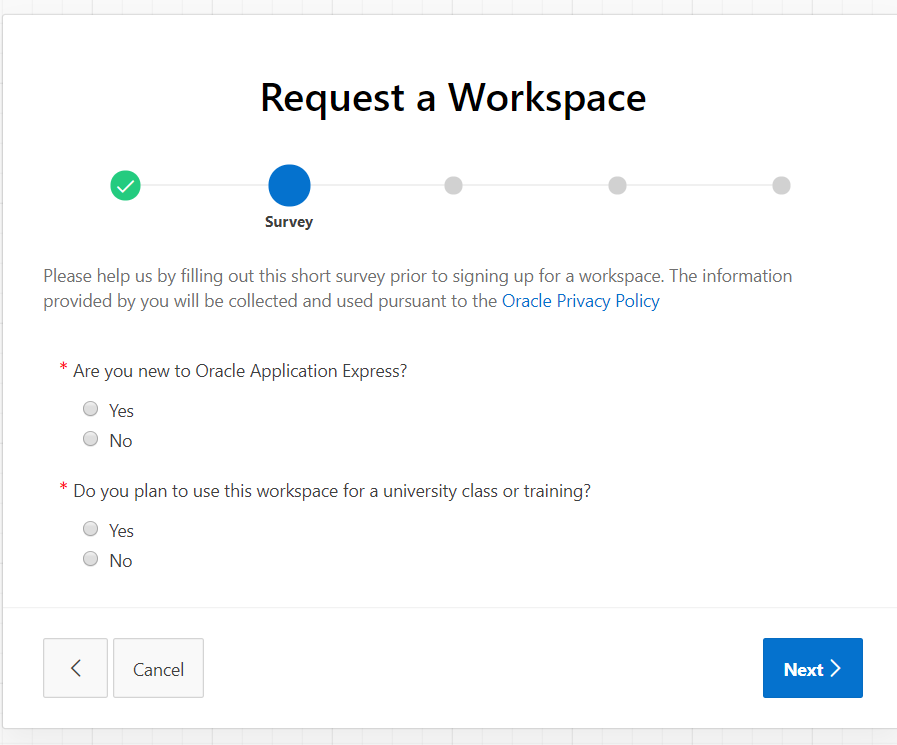
\includegraphics[scale=0.3]{figures/4.png}
    \label{4}
\end{figure}


\item \textbf{Isi alasan anda melakukan request workspace di APEX}
\begin{figure}[H]
    \centering
    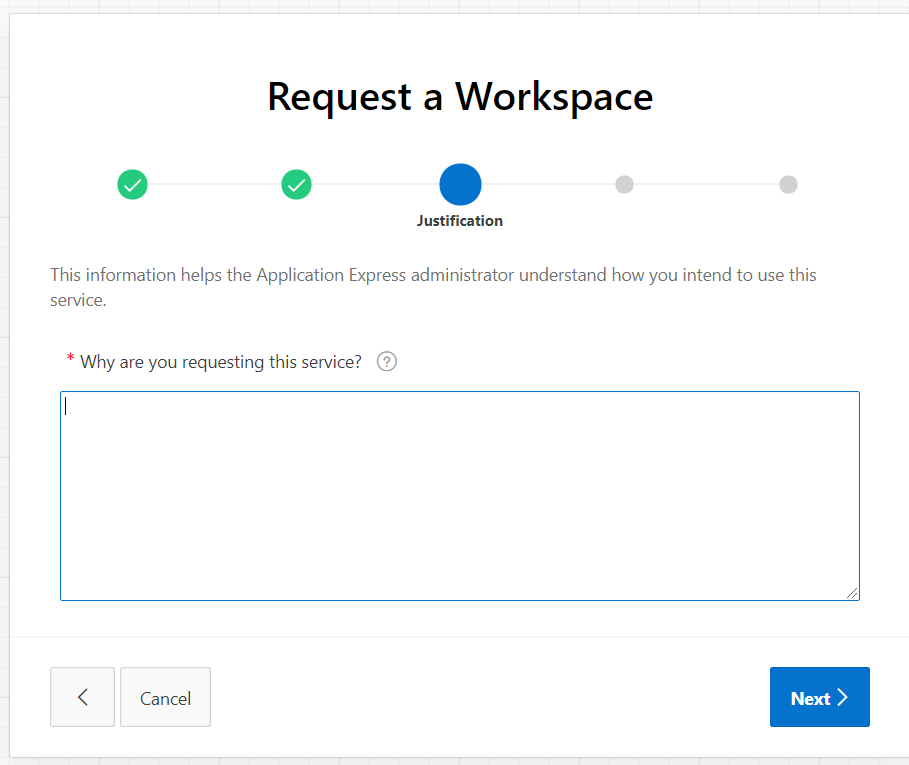
\includegraphics[scale=0.3]{figures/5.png}
    \label{5}
\end{figure}


\item \textbf{Lalu setujui laman persetujuan yang disediakan oleh oracle}
\begin{figure}[H]
    \centering
    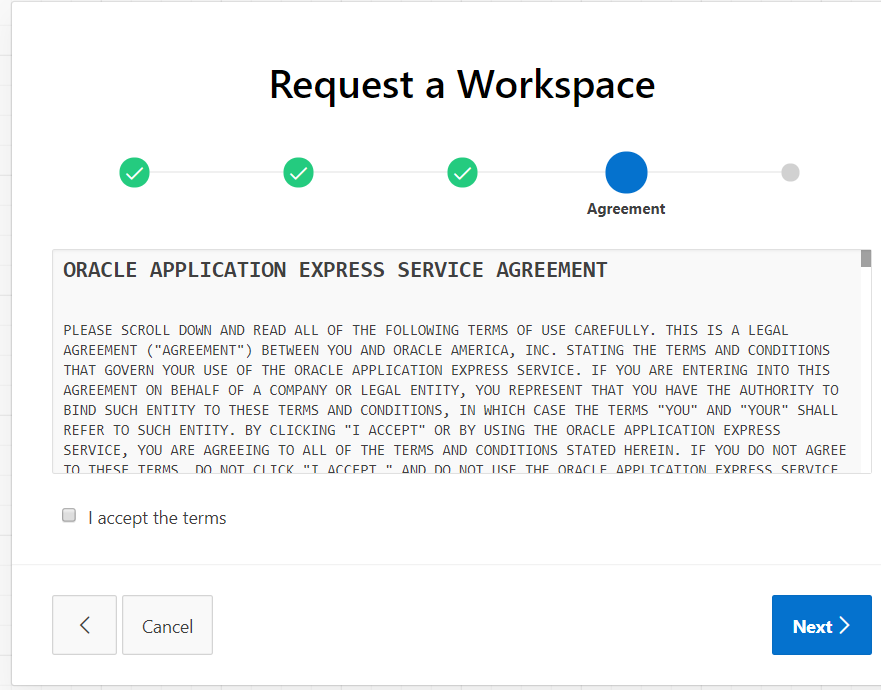
\includegraphics[scale=0.3]{figures/6.png}
    \label{6}
\end{figure}


\item \textbf{Setelah itu cek email anda, jika anda mendapatkan email dari oracle, klik Create Workspace yang berada pada email tersebut}
\begin{figure}[H]
    \centering
    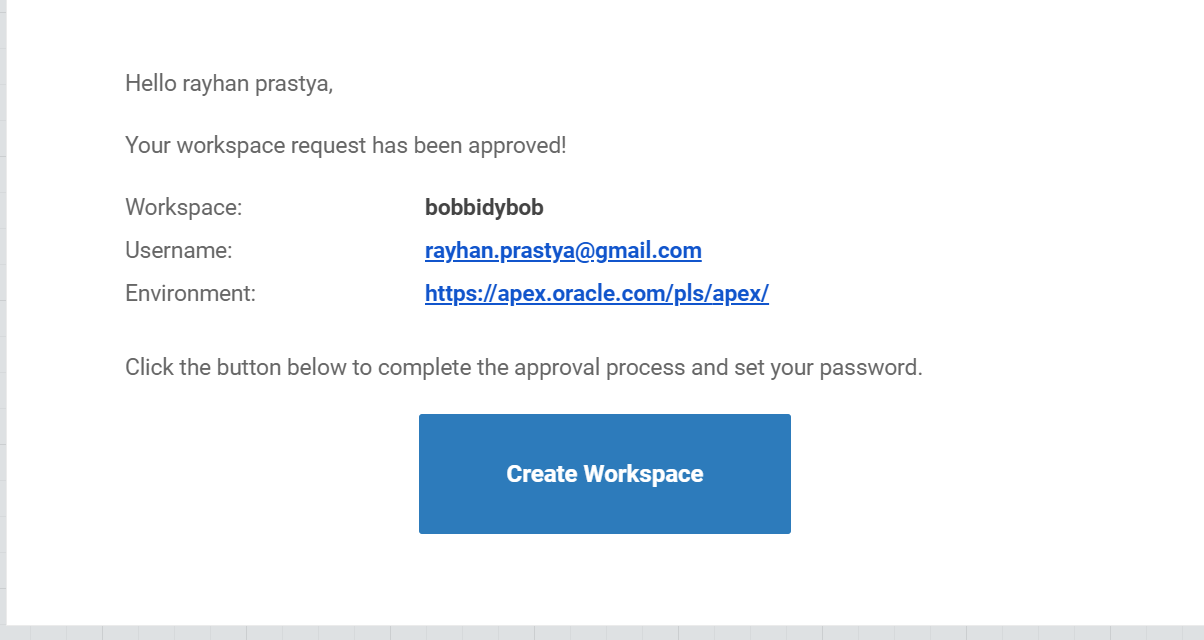
\includegraphics[scale=0.3]{figures/7.png}
    \label{7}
\end{figure}


\item \textbf{Input data pada form login APEX workspace}\begin{figure}[H]
    \centering
    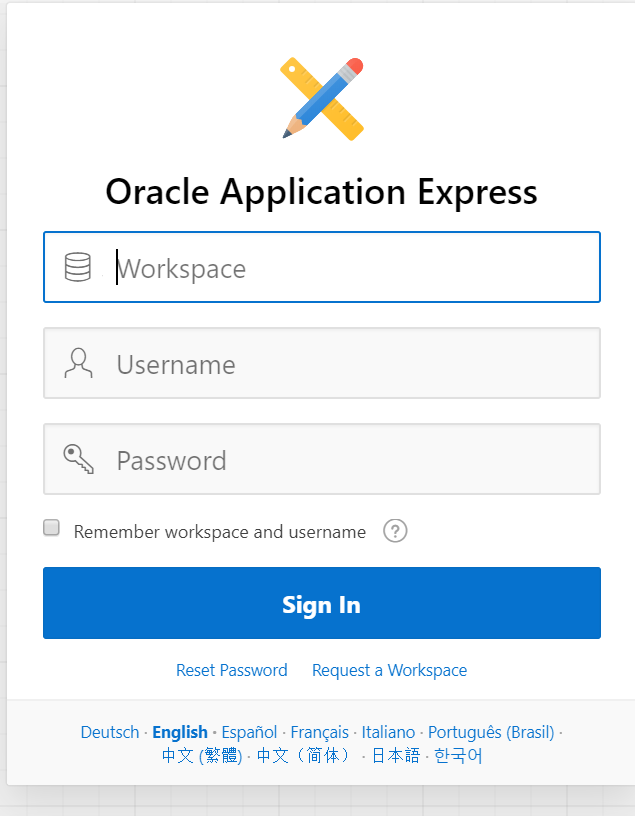
\includegraphics[scale=0.3]{figures/8.png}
    \label{8}
\end{figure}


\item \textbf{Setelah masuk ke laman menu, pilih menu app builder}\begin{figure}[H]
    \centering
    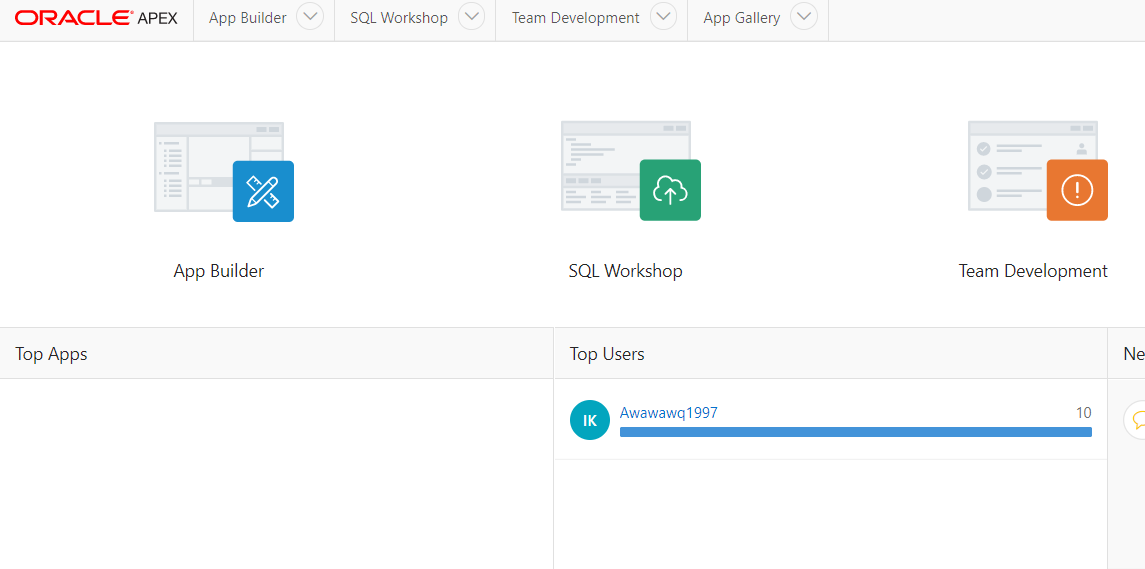
\includegraphics[scale=0.3]{figures/9.png}
    \label{9}
\end{figure}


\item \textbf{Setelah itu pilih create}\begin{figure}[H]
    \centering
    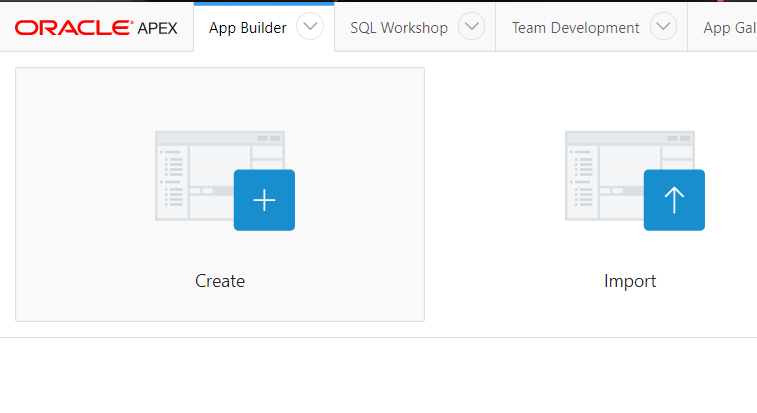
\includegraphics[scale=0.3]{figures/10.png}
    \label{10}
\end{figure}


\item \textbf{Anda akan dialihkan ke halaman pembuatan aplikasi, pilih menu From a File untuk mengupload data yang sudah dibuat(ekstensi file yang diupload harus berupa CSV,XLSX,XML, atau JSON.)}
\begin{figure}[H]
    \centering
    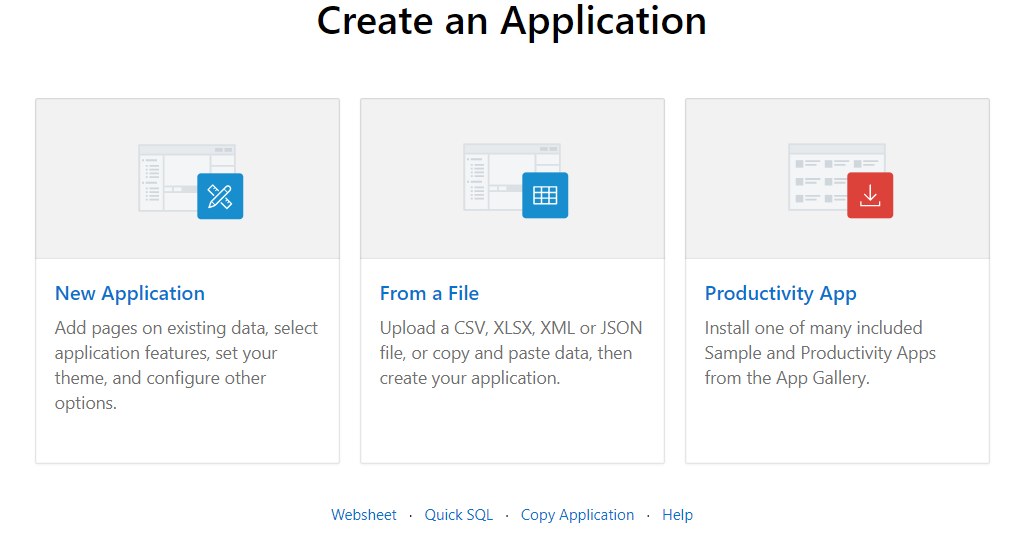
\includegraphics[scale=0.3]{figures/11.png}
    \label{11}
\end{figure}


\item \textbf{Masukkan file yang sudah anda buat sebelumnya}
\begin{figure}[H]
    \centering
    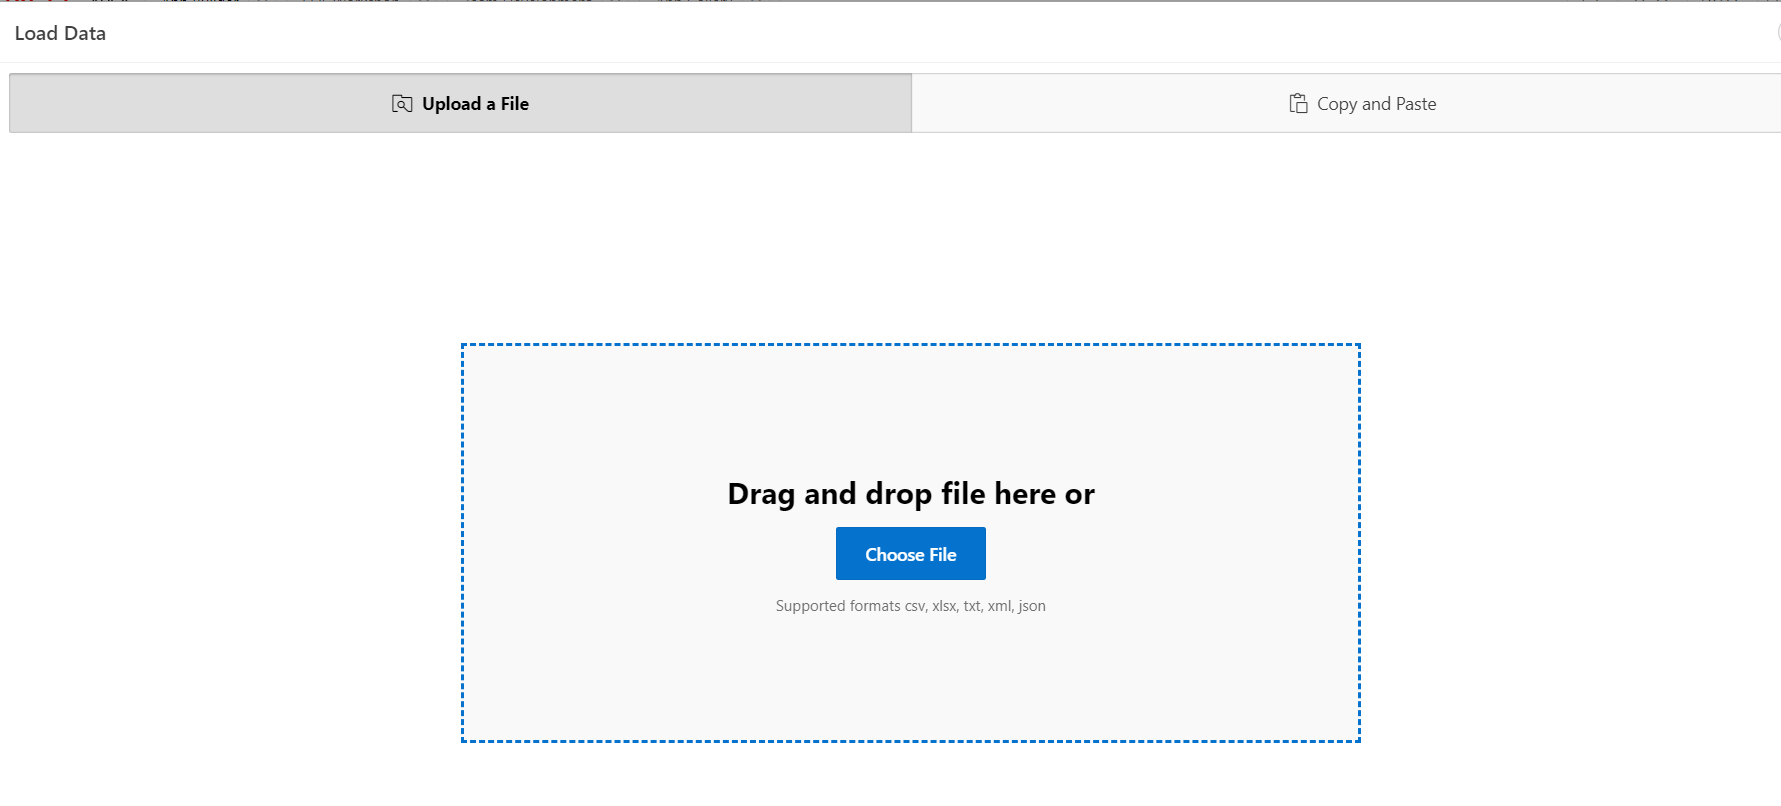
\includegraphics[scale=0.3]{figures/14.png}
    \label{12}
\end{figure}


\item \textbf{Setelah itu beri nama pada tabel yang telah diinputkan tadi, setelah selesai pilih load data}
\begin{figure}[H]
    \centering
    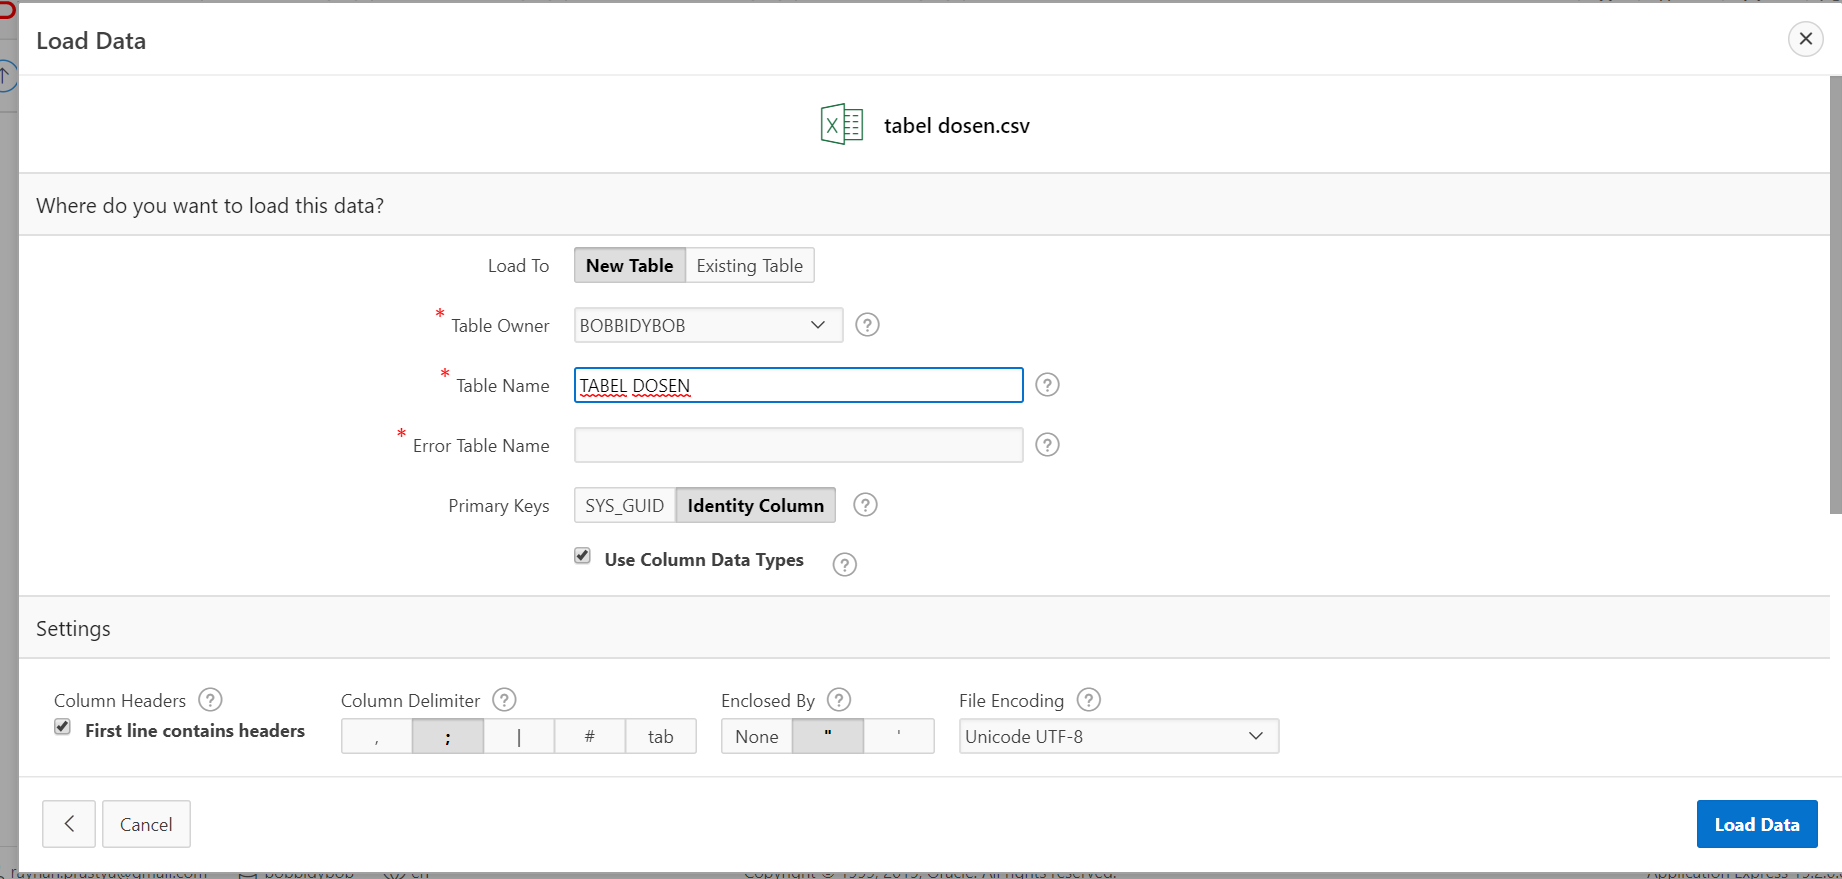
\includegraphics[scale=0.3]{figures/15.png}
    \label{13}
\end{figure}


\item \textbf{Lakukan hal yang sama jika anda masih memiliki data tabel yang ingin diinputkan}

\item \textbf{Jka dirasa cukup, pilih Create Application}
\begin{figure}[H]
    \centering
    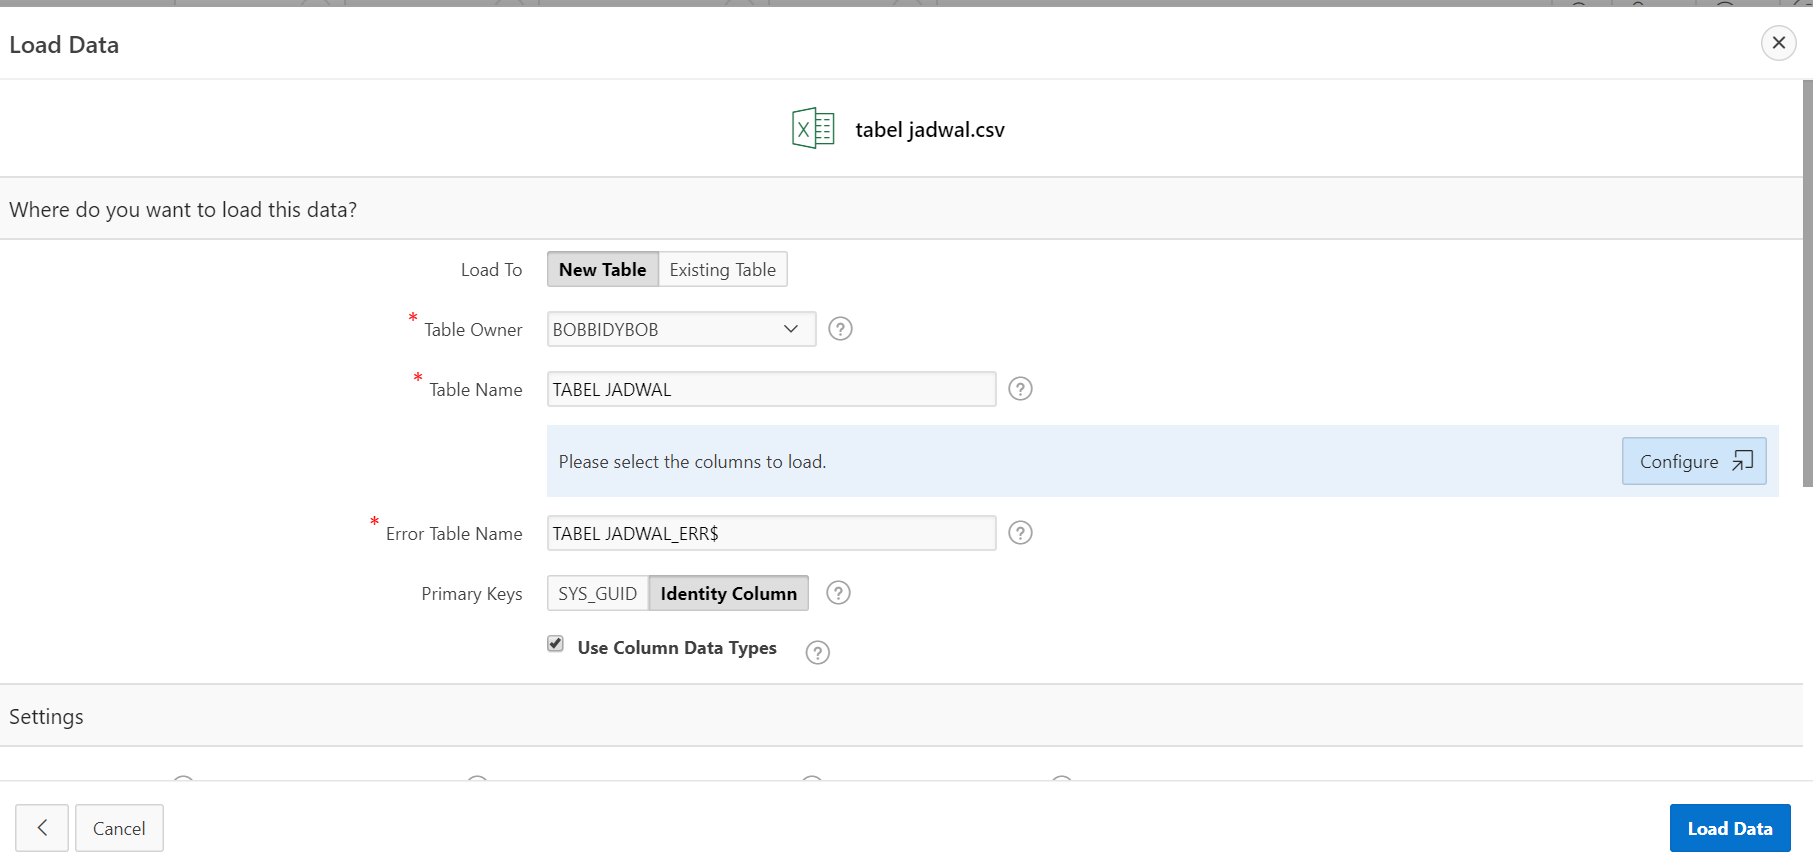
\includegraphics[scale=0.3]{figures/16.png}
    \label{14}
\end{figure}


\item \textbf{Lalu pilih Add page}
\begin{figure}[H]
    \centering
    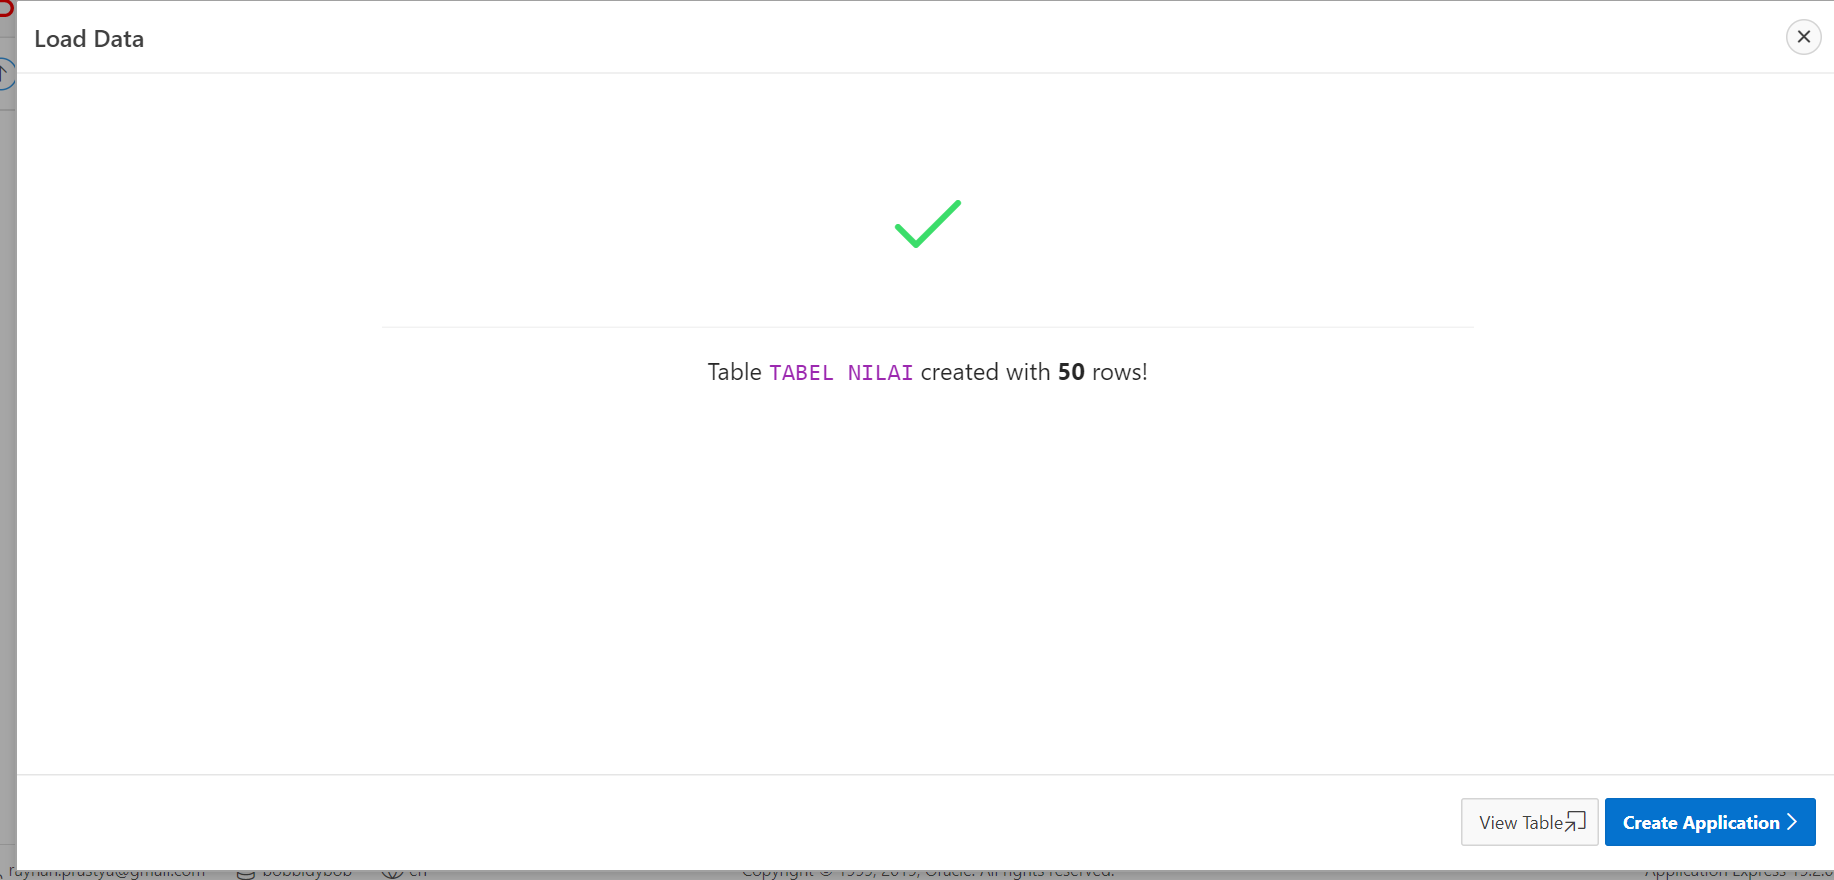
\includegraphics[scale=0.3]{figures/17.png}
    \label{15}
\end{figure}

\end{enumerate}
\section{Mengatur Primary Key}

Setelah melakukan hal-hal diatas, kita harus merelasikan tabel tabel yang sudah diinputkan. Command SQL yang digunakan adalah \textbf{ALTER}, ALTER berfungsi untuk mengubah struktur tabel pada suatu database.
\par 
Sebuah database akan diberikan primary key default berupa ID. kita dapat menghilangkan primary key default tersebut menggunakan command ALTER , contoh \textbf{alter table drop tabel\_mahasiswa column id } yang berarti kolom ID pada tabel mahasiswa akan dihilangkan.
\par
Selanjutnya adalah melakukan setting Primary key, Setelah menghapus kolom id maka posisi primary key pada masing masing tabel pun hilang, maka kita harus memasukkan primary key yang baru, salah satu ciri-ciri priamry key adalah berbeda dari yang lain, sehingga kita harus mencari suatu pembeda dari masing masing tabel untuk dijadikan primary key. Misalkan pada tabel mahasiswa memiliki kolom nim. Nim ini tidak dimiliki tabel-tabel yang lain atau bisa dibilang NIM ini dapat mewakili tabel mahasiswa dan bisa dijadikan primary key, cara menggunakannya adalah\\
\textbf{alter table tabel\_mahasiswa}\\
\textbf{add primary key (nim);}\\

\section{Interface}
\begin{enumerate}
\item \textbf{Pilih interface yang akan digunakan pada data tabel anda, disini saya menggunakan interface interactive report}
\begin{figure}[H]
    \centering
    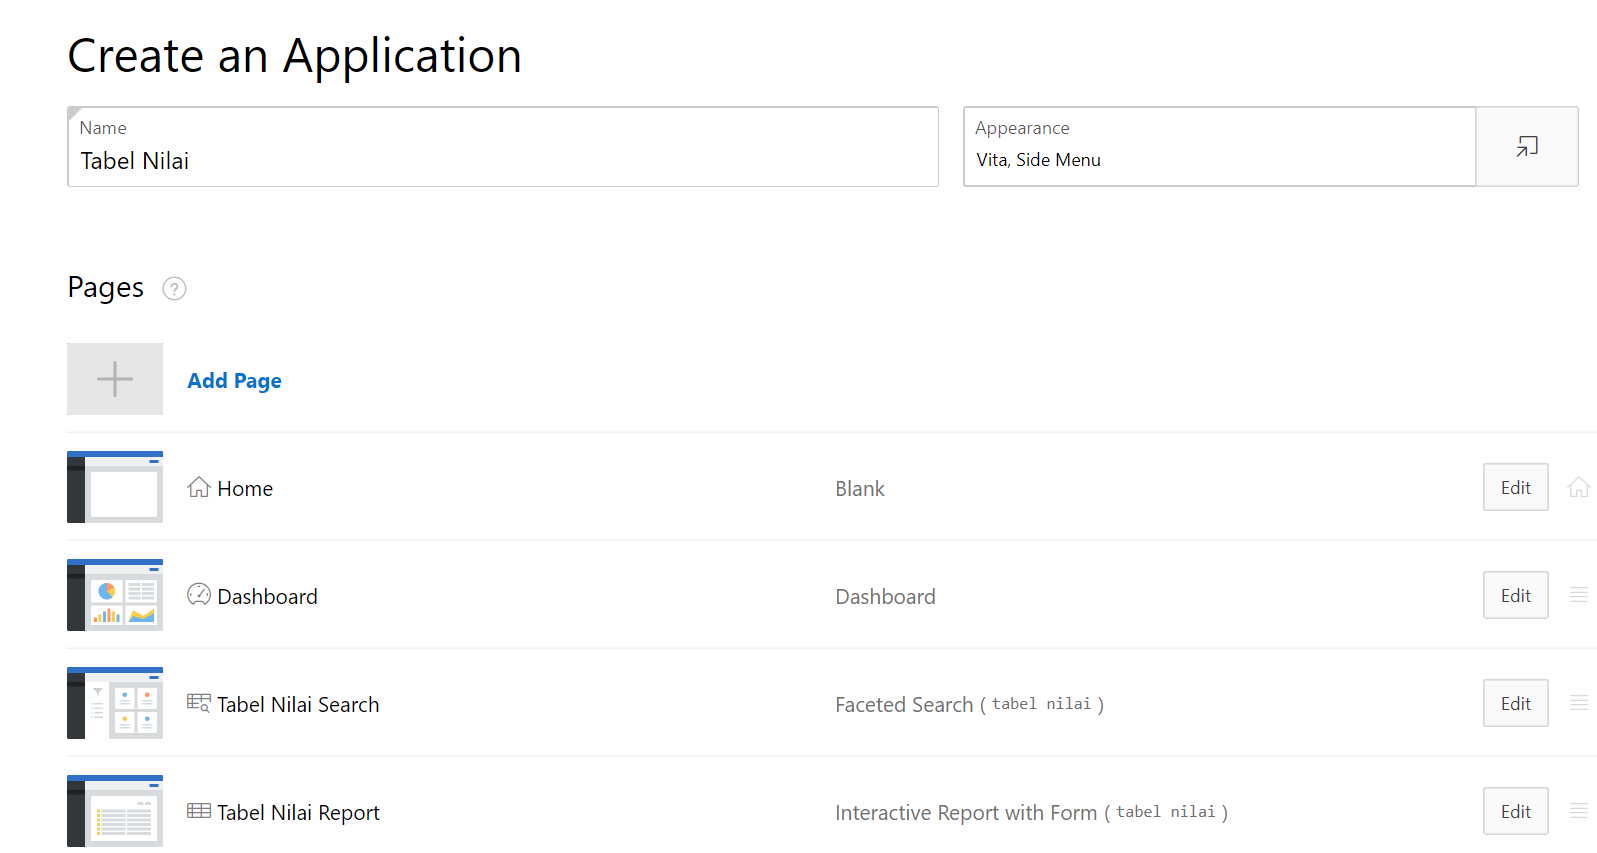
\includegraphics[scale=0.3]{figures/18.png}
    \label{16}
\end{figure}


\item \textbf{Berikan nama pada page yang nantinya akan dibuat}
\begin{figure}[H]
    \centering
    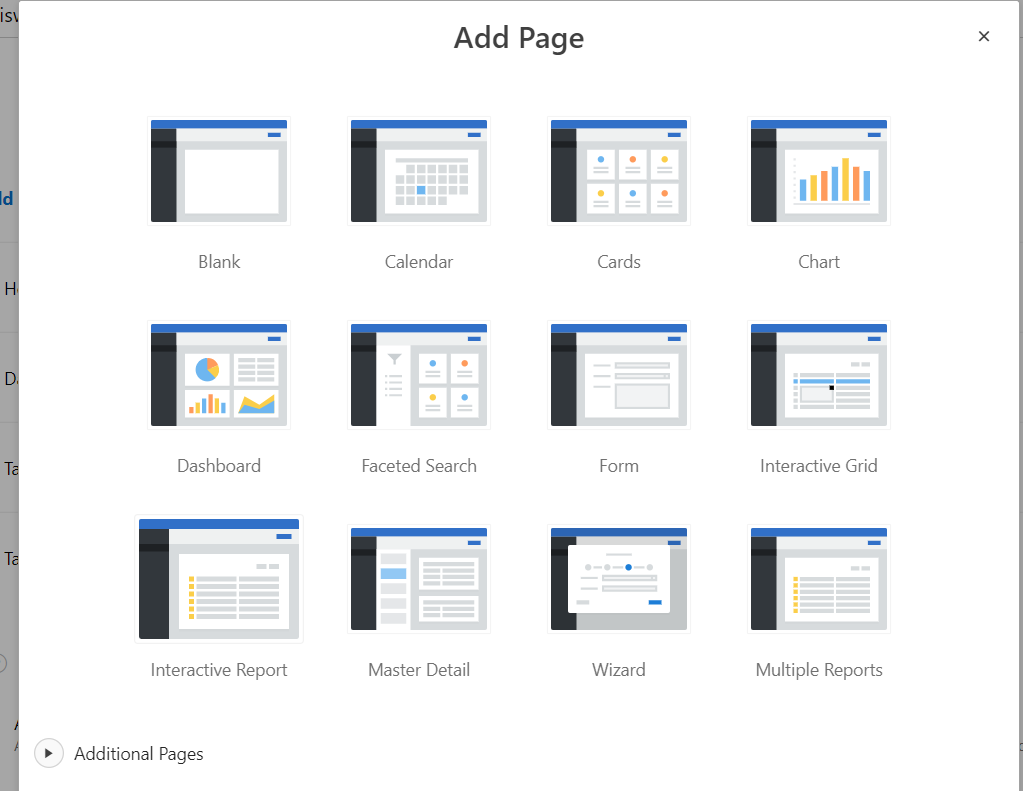
\includegraphics[scale=0.3]{figures/19.png}
    \label{17}
\end{figure}


\item \textbf{Lakukan hal serupa pada tabel-tabel yang telah anda inputkan}
\begin{figure}[H]
    \centering
    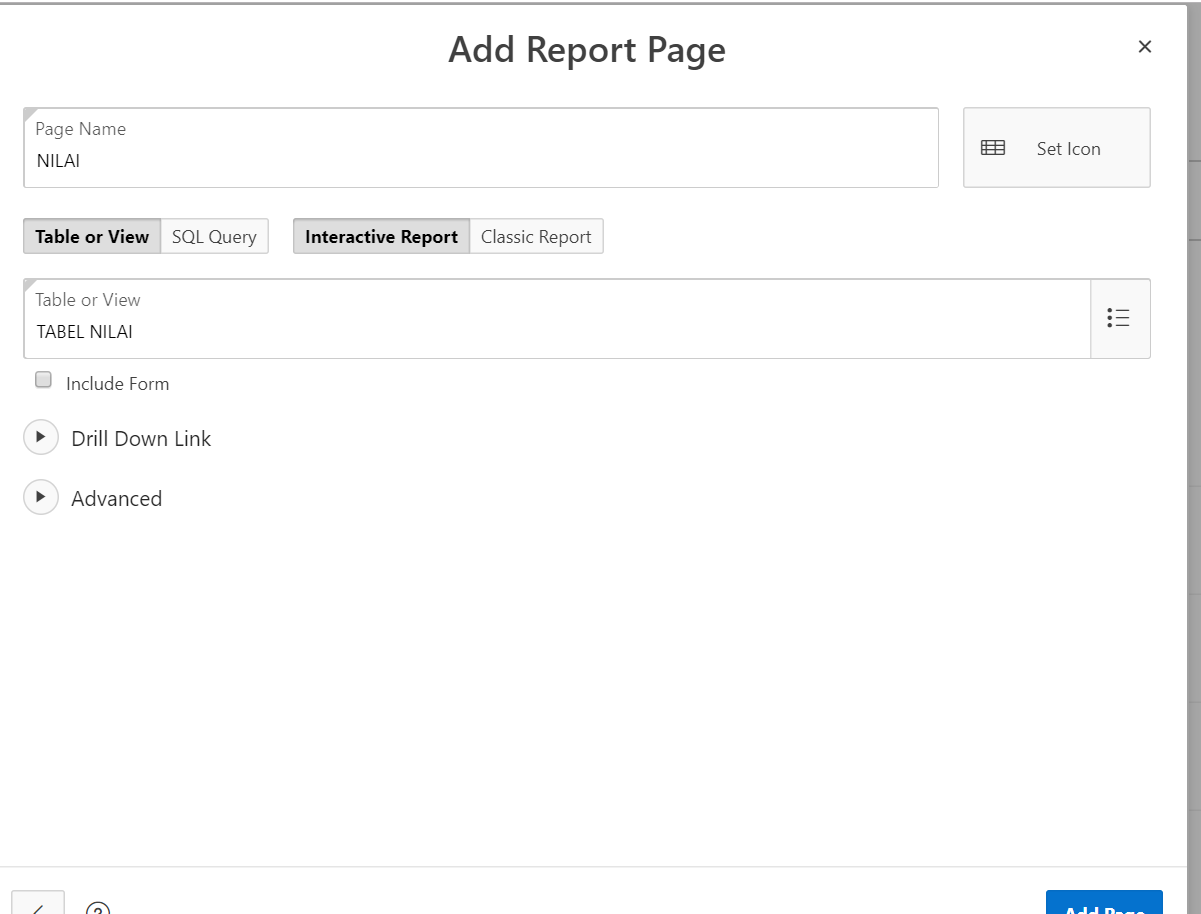
\includegraphics[scale=0.3]{figures/20.png}
    \label{18}
\end{figure}


\item \textbf{Lalu pilih menu create application}\begin{figure}[H]
    \centering
    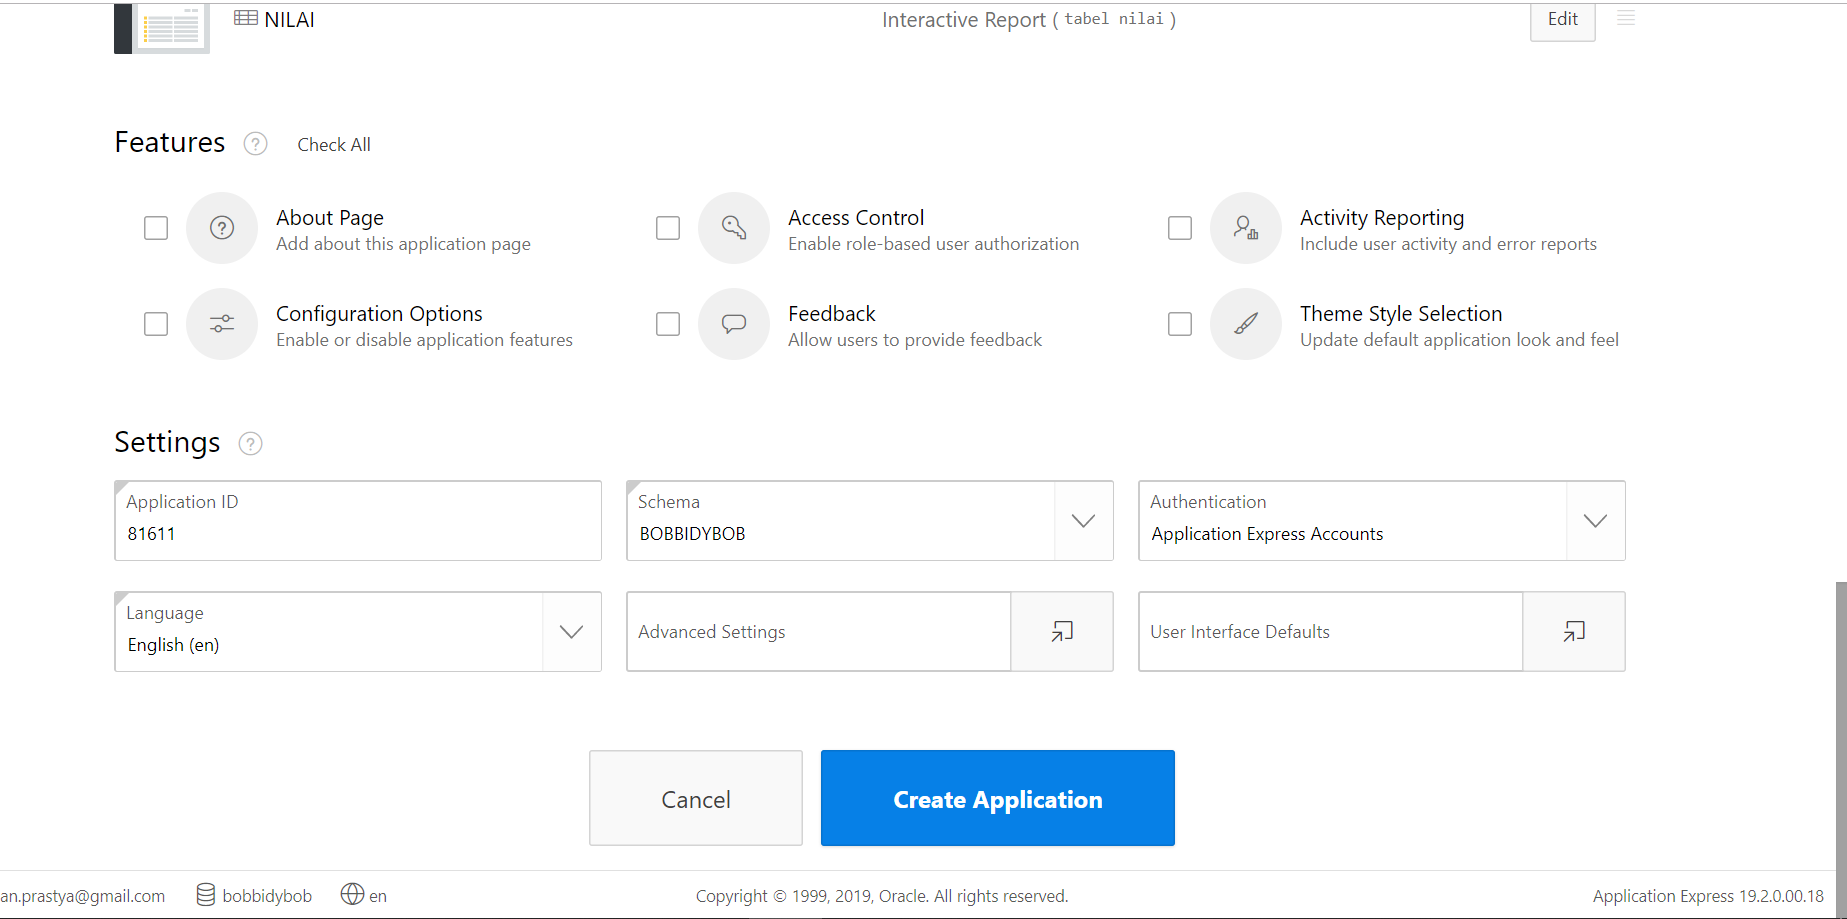
\includegraphics[scale=0.3]{figures/21.png}
    \label{19}
\end{figure}

\item \textbf{Aplikasi pun berhasil dibuat}
\begin{figure}[H]
    \centering
    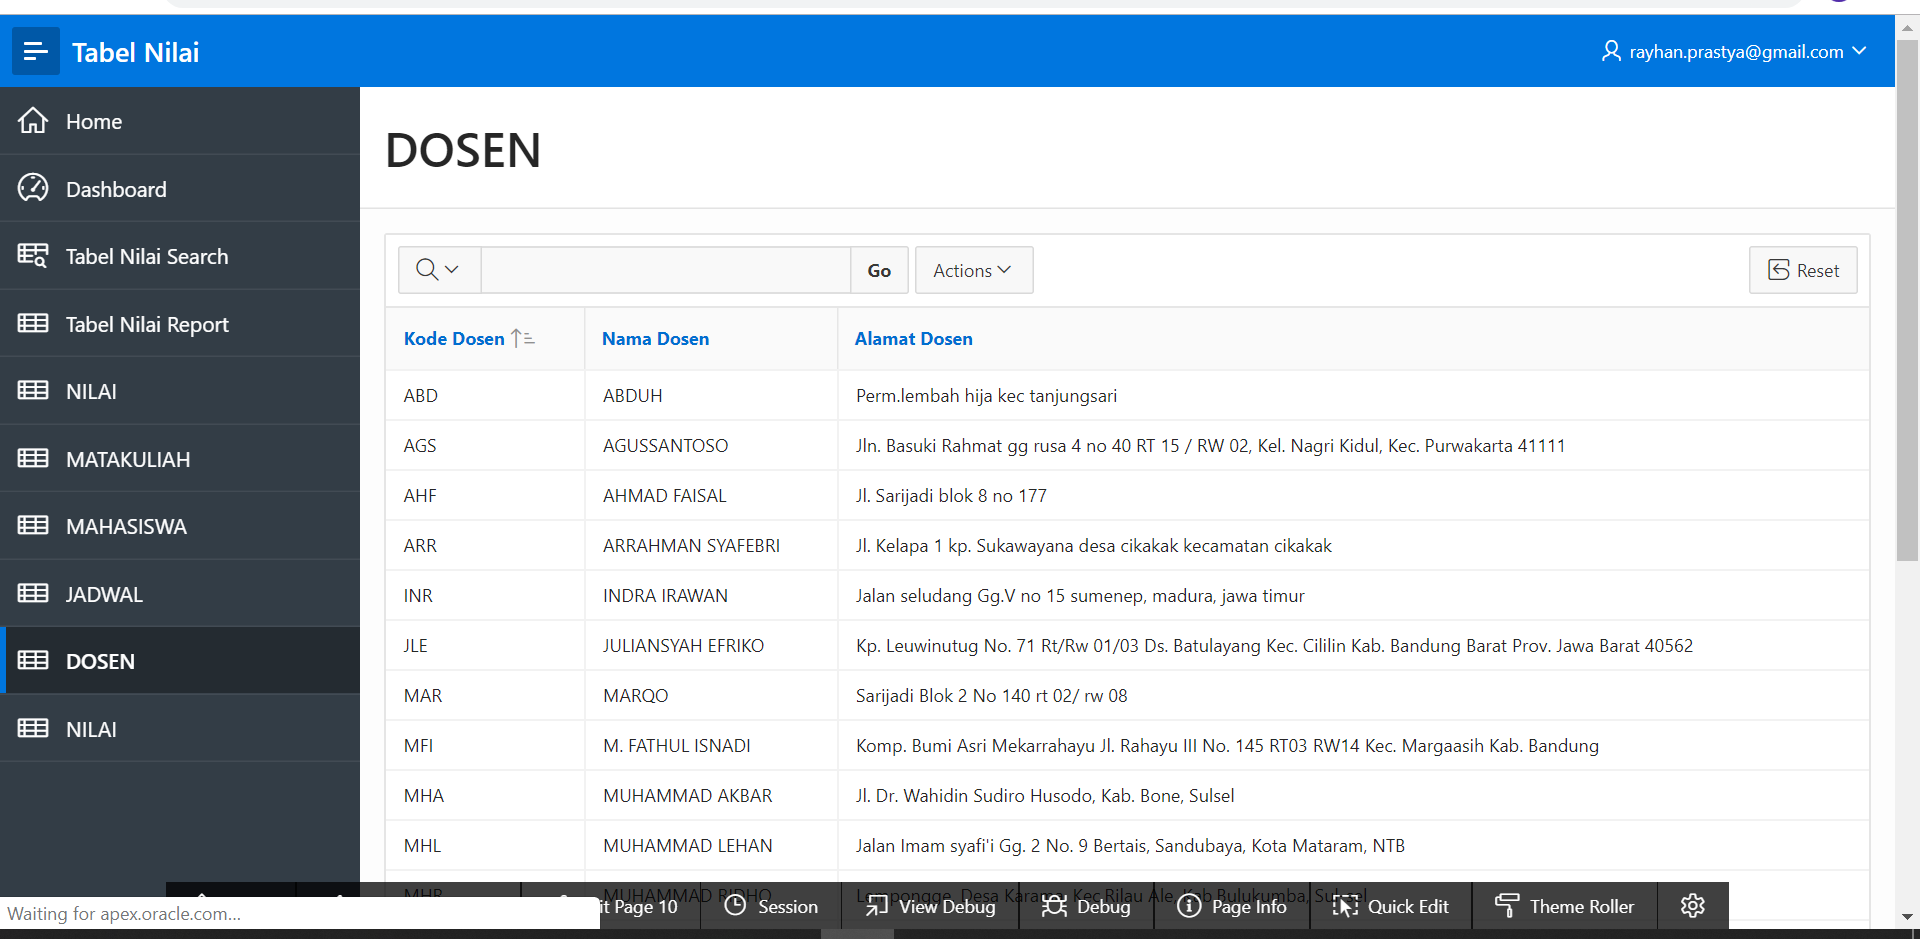
\includegraphics[scale=0.3]{figures/22.png}
    \label{28}
\end{figure}

\textbf{Workspace:} BOBBIDYBOB \\
\textbf{Username :} rayhan.prastya@gmail.com \\
\textbf{Password :} Prastya123

\end{enumerate}